% Created 2017-09-14 Thu 17:52
% Intended LaTeX compiler: pdflatex
\documentclass[11pt]{article}
\usepackage[utf8]{inputenc}
\usepackage[T1]{fontenc}
\usepackage{graphicx}
\usepackage{grffile}
\usepackage{longtable}
\usepackage{wrapfig}
\usepackage{rotating}
\usepackage[normalem]{ulem}
\usepackage{amsmath}
\usepackage{textcomp}
\usepackage{amssymb}
\usepackage{capt-of}
\usepackage{hyperref}
\usepackage{amsmath}
\usepackage{amsmath}
\author{Jake Brawer}
\date{\today}
\title{Assignment 1}
\hypersetup{
 pdfauthor={Jake Brawer},
 pdftitle={Assignment 1},
 pdfkeywords={},
 pdfsubject={},
 pdfcreator={Emacs 25.2.1 (Org mode 9.1)}, 
 pdflang={English}}
\begin{document}

\maketitle

\section*{Problem 1}
\label{sec:org29f5a92}
\subsection*{a)}
\label{sec:org672cbc1}

\subsubsection*{Solution}
\label{sec:orged64820}

The Answer is: 
\begin{equation}
\cfrac{{{4}\choose{1}} {{13}\choose{2}} {{3}\choose{3}} 13^3}{{{52}\choose{5}}} = 0.2637455
\end{equation}

\subsubsection*{Breakdown}
\label{sec:orgc4c2790}

Given that there are 5 cards and only 4 suits, we are guaranteed to have a repeat. \({{4}\choose{1}}\) represents the number of ways to choose the repeated suit. \({{13}\choose{2}}\) represents the number of ways to choose the ranks of the repeated suit cards \emph{without} overcounting. \({{3}\choose{3}}\) represents the number of ways to choose the rest of the ranks (just one way, as the last three cards must each be one of the last three ranks). \(13^{3}\) represents the ways to choose the ranks for the rest of the cards. And finally we divide by the number of possible 5 card hands. 

\subsection*{b)}
\label{sec:orgd4c6719}


The Answer is: 
\begin{equation}
\cfrac{{{4}\choose{1}} {{13}\choose{3}} {{3}\choose{3}} 13^3 + {{4}\choose{2}} {{13}\choose{2}}^{2} {{2}\choose{2}} 13^{2}} {{{52}\choose{6}}} = 0.4264821
\end{equation}

\subsubsection*{Breakdown}
\label{sec:org119f212}

The two multiplicative sequences (separated by addition) can be seen to represent two different "cases" which I will outline below.

\begin{itemize}
\item Case 1: Three cards share the same rank
\label{sec:org92897a5}

\({4}\choose{1}\) represents the number of ways of choosing the suit for the three cards. \({{13}\choose{3}}\) represents the number of ways of choosing the ranks for these 3 cards of the same suit. \({{3}\choose{3}}\) represents the number of ways to choose the rest of the ranks (just one way, as the last three cards must each be one of the last three ranks). \(13^{3}\) represents the ways to choose the ranks for the rest of the cards. And finally we divide by the number of possible 5 card hands.

\item Case 2: Two sets of two cards each share the same rank
\label{sec:orgfdb33ff}

\({4}\choose{2}\) represents the number of ways of choosing the two suits for the four cards. \({{13}\choose{2}}^{2}\) represents the number of ways of choosing the ranks for these 2 sets of cards of the same suit. \({{2}\choose{2}}\) represents the number of ways to choose the rest of the ranks (just one way, as the last two cards must each be one of the last three ranks). \(13^{2}\) represents the ways to choose the ranks for the rest of the cards. And finally we divide by the number of possible 6 card hands.
\end{itemize}

\section*{Problem 2: simulations}
\label{sec:org76c7cb4}

\begin{verbatim}
probAllSuits <- function(reps, handsize){

# Initialize the deck
  H <- rep("h", 13)
  S <- rep("s", 13)
  C <- rep("c", 13)
  D <- rep("d", 13)
  deck <- c(H,S,C,D)



  count <- 0 # Tracks number of hands w/ all ranks
  for (i in 1:reps){
  # samples handsize number of cards from the deck
    hand <- sample(deck, handsize, replace=FALSE)
    # if all ranks are present, increment counter
    if(length(table(hand)) == 4){
      count = count + 1
    }
  }

  sprintf("Probability of all suits appearing in %s-card 
             hand after %s reps: %s" ,
             handsize,
             reps,
             count / reps)

}


\end{verbatim}


\begin{verbatim}
probAllSuits(10000,5)
\end{verbatim}

\begin{center}
\begin{tabular}{l}
Probability of all suits appearing in 5-card\\
hand after 10000 reps: 0.2625\\
\end{tabular}
\end{center}

\begin{verbatim}
probAllSuits(10000,6)
\end{verbatim}

\begin{center}
\begin{tabular}{l}
Probability of all suits appearing in 6-card\\
hand after 10000 reps: 0.4321\\
\end{tabular}
\end{center}

\section*{Problem 3}
\label{sec:org728f752}
\subsection*{a)}
\label{sec:org1d293bf}

\text{To me this sounds like the following:\\}
\begin{equation}
  \begin{align}
    P(A \Delta B) = P(A \cup B) - P(A \cap B)
    \end{align}
\end{equation}
\text{From the notes we have:\\}
\begin{equation}
  \begin{align}
    P(A \cup B) = P(A) + P(B) - P(A \cap B)
    \end{align}
\end{equation}

\text{Therefore:\\}
\begin{equation}
  \begin{align}
    P(A \Delta B) = P(A) + P(B) - 2P(A \cap B)
    \end{align}
\end{equation}

\subsection*{b)}
\label{sec:org89b8435}

From the problem we have:

\begin{equation}
\begin{align}
P(A\mid B) > P(A)
\end{align}
\end{equation}

This is equivalent to:

\begin{equation}
\begin{align}
  \frac{P(A \cap B)}{P(B)} > P(A)
\end{align}
\end{equation}

So \(P(A \cap B)\) must be positive. This can be rearranged to: 

\begin{equation}
\begin{align}
  \frac{P(A \cap B)}{P(A)} > P(B)
\end{align}
\end{equation}

Which is equivalent to:

\begin{equation}
\begin{align}
  \frac{P(A \cap B)}{P(B)} > P(A)
\end{align}
\end{equation}

Which implies:

\begin{equation}
\begin{align}
P(B\mid A) > P(B)
\end{align}
\end{equation}
Since we are given that \(P(B)\) is positive, and since \(P(A \cap B)\), we know this must be true.

\subsection*{c)}
\label{sec:orgb0e8e24}
\subsubsection*{A and B are disjoint}
\label{sec:org4c44328}
\begin{equation}
\begin{align}
 P(A \cup B) = P(A) + P(B)
\end{align}
\end{equation}
$\text{therefore:}$\\

\begin{equation}
\begin{align}
 0.9 = 0.6 + P(B)
\end{align}
\end{equation}
\begin{equation}
\begin{align}
 0.3 = P(B)
\end{align}
\end{equation}

\subsubsection*{A and B are independent}
\label{sec:org2bc1987}

\begin{equation}
\begin{align}
  P(A \cap B) = P(A)P(B)
\end{align}
\end{equation}
$\text{And also:}$\\
\begin{equation}
\begin{align}
  P(A \cup B) &= P(A) + P(B) - P(A \cap B)\\
  &= P(A) + P(B) - P(A)P(B)\\
  &= P(A) + P(B)\left(1 - P(A))\right\\
\end{align}
\end{equation}
$\text{Plugging in the values we get:}$\\
\begin{equation}
\begin{align}
  0.9 &= 0.6 + P(B)\left(0.4)\right\\
  &= 0.75 = P(B)
\end{align}
\end{equation}

\section*{Problem 4}
\label{sec:orgba81189}
\subsection*{a)}
\label{sec:orgc6ce89b}

\begin{verbatim}

# create arithmetic sequences
logprobs <- rep(1,365)
for(k in 1:365){
  factors <- seq(from = 365,length.out= k, by = -1)
  prob <- prod(factors) / (365^k)
  if(is.nan(prob)){
    logprobs[k] <- logprobs[k-1]  + log10(tail(factors, 1) / 365)
  }
  logprobs[k] <- log10(prob)
}

logprobs[1:100]
\end{verbatim}

\begin{center}
\begin{tabular}{r}
0\\
-0.00119148080741871\\
-0.00357772022778088\\
-0.00716201415108991\\
-0.0119476767019067\\
-0.0179380403910941\\
-0.0251364562692497\\
-0.03354629408185\\
-0.0431709424261316\\
-0.054013808909731\\
-0.0660783203111117\\
-0.0793679227417985\\
-0.0938860818104507\\
-0.109636282788794\\
-0.126622030779445\\
-0.144846850885644\\
-0.164314288382939\\
-0.185027908892833\\
-0.206991298558434\\
-0.230208064222132\\
-0.254681833605332\\
-0.280416255490277\\
-0.307414999903981\\
-0.335681758304321\\
-0.365220243768298\\
-0.396034191182517\\
-0.42812735743591\\
-0.46150352161473\\
-0.496166485199866\\
-0.532120072266497\\
-0.569368129686126\\
-0.607914527331036\\
-0.647763158281191\\
-0.68891793903363\\
-0.731382809714386\\
-0.775161734292973\\
-0.820258700799473\\
-0.866677721544269\\
-0.914422833340457\\
-0.963498097728993\\
-1.01390760120659\\
-1.06565545545646\\
-1.11874579758183\\
-1.17318279034247\\
-1.22897062239407\\
-1.28611350853064\\
-1.34461568992994\\
-1.40448143440198\\
-1.4657150366407\\
-1.52832081847877\\
-1.59230312914565\\
-1.65766634552891\\
-1.72441487243893\\
-1.79255314287696\\
-1.8620856183066\\
-1.9330167889288\\
-2.00535117396044\\
-2.07909332191647\\
-2.15424781089576\\
-2.23081924887066\\
-2.30881227398035\\
-2.38823155482807\\
-2.46908179078224\\
-2.55136771228156\\
-2.63509408114419\\
-2.720265690881\\
-2.80688736701305\\
-2.89496396739327\\
-2.98450038253253\\
-3.07550153593007\\
-3.16797238440838\\
-3.2619179184527\\
-3.35734316255506\\
-3.45425317556312\\
-3.55265305103369\\
-3.6525479175912\\
-3.75394293929113\\
-3.85684331598838\\
-3.96125428371086\\
-4.06718111503829\\
-4.17462911948625\\
-4.28360364389569\\
-4.39411007282788\\
-4.50615382896499\\
-4.61974037351638\\
-4.73487520663064\\
-4.85156386781352\\
-4.96981193635192\\
-5.08962503174394\\
-5.2110088141352\\
-5.33396898476141\\
-5.4585112863975\\
-5.58464150381322\\
-5.71236546423549\\
-5.84168903781756\\
-5.97261813811505\\
-6.10515872256911\\
-6.2393167929968\\
-6.3750983960887\\
-6.51250962391411\\
\end{tabular}
\end{center}

\subsection*{b)}
\label{sec:org2c3c953}

\section*{Problem 1}
\label{sec:orga78a944}
\subsection*{a)}
\label{sec:org894ba6b}

\subsubsection*{Solution}
\label{sec:orgda37004}

The Answer is: 
\begin{equation}
\cfrac{{{4}\choose{1}} {{13}\choose{2}} {{3}\choose{3}} 13^3}{{{52}\choose{5}}} = 0.2637455
\end{equation}

\subsubsection*{Breakdown}
\label{sec:org789e395}

Given that there are 5 cards and only 4 suits, we are guaranteed to have a repeat. \({{4}\choose{1}}\) represents the number of ways to choose the repeated suit. \({{13}\choose{2}}\) represents the number of ways to choose the ranks of the repeated suit cards \emph{without} overcounting. \({{3}\choose{3}}\) represents the number of ways to choose the rest of the ranks (just one way, as the last three cards must each be one of the last three ranks). \(13^{3}\) represents the ways to choose the ranks for the rest of the cards. And finally we divide by the number of possible 5 card hands. 

\subsection*{b)}
\label{sec:orgbcccff4}


The Answer is: 
\begin{equation}
\cfrac{{{4}\choose{1}} {{13}\choose{3}} {{3}\choose{3}} 13^3 + {{4}\choose{2}} {{13}\choose{2}}^{2} {{2}\choose{2}} 13^{2}} {{{52}\choose{6}}} = 0.4264821
\end{equation}

\subsubsection*{Breakdown}
\label{sec:orgda1da68}

The two multiplicative sequences (separated by addition) can be seen to represent two different "cases" which I will outline below.

\begin{itemize}
\item Case 1: Three cards share the same rank
\label{sec:org07b351d}

\({4}\choose{1}\) represents the number of ways of choosing the suit for the three cards. \({{13}\choose{3}}\) represents the number of ways of choosing the ranks for these 3 cards of the same suit. \({{3}\choose{3}}\) represents the number of ways to choose the rest of the ranks (just one way, as the last three cards must each be one of the last three ranks). \(13^{3}\) represents the ways to choose the ranks for the rest of the cards. And finally we divide by the number of possible 5 card hands.

\item Case 2: Two sets of two cards each share the same rank
\label{sec:org745c3c3}

\({4}\choose{2}\) represents the number of ways of choosing the two suits for the four cards. \({{13}\choose{2}}^{2}\) represents the number of ways of choosing the ranks for these 2 sets of cards of the same suit. \({{2}\choose{2}}\) represents the number of ways to choose the rest of the ranks (just one way, as the last two cards must each be one of the last three ranks). \(13^{2}\) represents the ways to choose the ranks for the rest of the cards. And finally we divide by the number of possible 6 card hands.
\end{itemize}

\section*{Problem 2: simulations}
\label{sec:orgc2c6337}

\begin{verbatim}
probAllSuits <- function(reps, handsize){

# Initialize the deck
  H <- rep("h", 13)
  S <- rep("s", 13)
  C <- rep("c", 13)
  D <- rep("d", 13)
  deck <- c(H,S,C,D)



  count <- 0 # Tracks number of hands w/ all ranks
  for (i in 1:reps){
  # samples handsize number of cards from the deck
    hand <- sample(deck, handsize, replace=FALSE)
    # if all ranks are present, increment counter
    if(length(table(hand)) == 4){
      count = count + 1
    }
  }

  sprintf("Probability of all suits appearing in %s-card 
             hand after %s reps: %s" ,
             handsize,
             reps,
             count / reps)

}


\end{verbatim}


\begin{verbatim}
probAllSuits(10000,5)
\end{verbatim}

\begin{center}
\begin{tabular}{l}
Probability of all suits appearing in 5-card\\
hand after 10000 reps: 0.2747\\
\end{tabular}
\end{center}

\begin{verbatim}
probAllSuits(10000,6)
\end{verbatim}

\begin{center}
\begin{tabular}{l}
Probability of all suits appearing in 6-card\\
hand after 10000 reps: 0.4203\\
\end{tabular}
\end{center}

\section*{Problem 3}
\label{sec:org4436f84}
\subsection*{a)}
\label{sec:org57fc108}

\text{To me this sounds like the following:\\}
\begin{equation}
  \begin{align}
    P(A \Delta B) = P(A \cup B) - P(A \cap B)
    \end{align}
\end{equation}
\text{From the notes we have:\\}
\begin{equation}
  \begin{align}
    P(A \cup B) = P(A) + P(B) - P(A \cap B)
    \end{align}
\end{equation}

\text{Therefore:\\}
\begin{equation}
  \begin{align}
    P(A \Delta B) = P(A) + P(B) - 2P(A \cap B)
    \end{align}
\end{equation}

\subsection*{b)}
\label{sec:org3688b54}

From the problem we have:

\begin{equation}
\begin{align}
P(A\mid B) > P(A)
\end{align}
\end{equation}

This is equivalent to:

\begin{equation}
\begin{align}
  \frac{P(A \cap B)}{P(B)} > P(A)
\end{align}
\end{equation}

So \(P(A \cap B)\) must be positive. This can be rearranged to: 

\begin{equation}
\begin{align}
  \frac{P(A \cap B)}{P(A)} > P(B)
\end{align}
\end{equation}

Which is equivalent to:

\begin{equation}
\begin{align}
  \frac{P(A \cap B)}{P(B)} > P(A)
\end{align}
\end{equation}

Which implies:

\begin{equation}
\begin{align}
P(B\mid A) > P(B)
\end{align}
\end{equation}
Since we are given that \(P(B)\) is positive, and since \(P(A \cap B)\), we know this must be true.

\subsection*{c)}
\label{sec:org3cb7128}
\subsubsection*{A and B are disjoint}
\label{sec:org24aa3b5}
\begin{equation}
\begin{align}
 P(A \cup B) = P(A) + P(B)
\end{align}
\end{equation}
$\text{therefore:}$\\

\begin{equation}
\begin{align}
 0.9 = 0.6 + P(B)
\end{align}
\end{equation}
\begin{equation}
\begin{align}
 0.3 = P(B)
\end{align}
\end{equation}

\subsubsection*{A and B are independent}
\label{sec:org3fa9522}

\begin{equation}
\begin{align}
  P(A \cap B) = P(A)P(B)
\end{align}
\end{equation}
$\text{And also:}$\\
\begin{equation}
\begin{align}
  P(A \cup B) &= P(A) + P(B) - P(A \cap B)\\
  &= P(A) + P(B) - P(A)P(B)\\
  &= P(A) + P(B)\left(1 - P(A))\right\\
\end{align}
\end{equation}
$\text{Plugging in the values we get:}$\\
\begin{equation}
\begin{align}
  0.9 &= 0.6 + P(B)\left(0.4)\right\\
  &= 0.75 = P(B)
\end{align}
\end{equation}

\section*{Problem 4}
\label{sec:org0614363}
\subsection*{a)}
\label{sec:org8f80a17}

\begin{verbatim}

# create arithmetic sequences
logprobs <- rep(1,365)
for(k in 1:365){
  factors <- seq(from = 365,length.out= k, by = -1)
  prob <- prod(factors) / (365^k)
  if(is.nan(prob)){
    logprobs[k] <- logprobs[k-1]  + log10(tail(factors, 1) / 365)
  }
  logprobs[k] <- log10(prob)
}

logprobs[1:100]
\end{verbatim}

\begin{center}
\begin{tabular}{r}
0\\
-0.00119148080741871\\
-0.00357772022778088\\
-0.00716201415108991\\
-0.0119476767019067\\
-0.0179380403910941\\
-0.0251364562692497\\
-0.03354629408185\\
-0.0431709424261316\\
-0.054013808909731\\
-0.0660783203111117\\
-0.0793679227417985\\
-0.0938860818104507\\
-0.109636282788794\\
-0.126622030779445\\
-0.144846850885644\\
-0.164314288382939\\
-0.185027908892833\\
-0.206991298558434\\
-0.230208064222132\\
-0.254681833605332\\
-0.280416255490277\\
-0.307414999903981\\
-0.335681758304321\\
-0.365220243768298\\
-0.396034191182517\\
-0.42812735743591\\
-0.46150352161473\\
-0.496166485199866\\
-0.532120072266497\\
-0.569368129686126\\
-0.607914527331036\\
-0.647763158281191\\
-0.68891793903363\\
-0.731382809714386\\
-0.775161734292973\\
-0.820258700799473\\
-0.866677721544269\\
-0.914422833340457\\
-0.963498097728993\\
-1.01390760120659\\
-1.06565545545646\\
-1.11874579758183\\
-1.17318279034247\\
-1.22897062239407\\
-1.28611350853064\\
-1.34461568992994\\
-1.40448143440198\\
-1.4657150366407\\
-1.52832081847877\\
-1.59230312914565\\
-1.65766634552891\\
-1.72441487243893\\
-1.79255314287696\\
-1.8620856183066\\
-1.9330167889288\\
-2.00535117396044\\
-2.07909332191647\\
-2.15424781089576\\
-2.23081924887066\\
-2.30881227398035\\
-2.38823155482807\\
-2.46908179078224\\
-2.55136771228156\\
-2.63509408114419\\
-2.720265690881\\
-2.80688736701305\\
-2.89496396739327\\
-2.98450038253253\\
-3.07550153593007\\
-3.16797238440838\\
-3.2619179184527\\
-3.35734316255506\\
-3.45425317556312\\
-3.55265305103369\\
-3.6525479175912\\
-3.75394293929113\\
-3.85684331598838\\
-3.96125428371086\\
-4.06718111503829\\
-4.17462911948625\\
-4.28360364389569\\
-4.39411007282788\\
-4.50615382896499\\
-4.61974037351638\\
-4.73487520663064\\
-4.85156386781352\\
-4.96981193635192\\
-5.08962503174394\\
-5.2110088141352\\
-5.33396898476141\\
-5.4585112863975\\
-5.58464150381322\\
-5.71236546423549\\
-5.84168903781756\\
-5.97261813811505\\
-6.10515872256911\\
-6.2393167929968\\
-6.3750983960887\\
-6.51250962391411\\
\end{tabular}
\end{center}

\subsection*{b)}
\label{sec:org4acd6c0}

\begin{verbatim}
lloydsFunc <- function(){
  for(k in 1:365){
    factors <- seq(from = 365,length.out= k, by = -1)
    prob <- prod(factors) / (365^k)
    if(!is.nan(prob)){
      if(prob <= 1e-6){
        return(k)
    }
  }
  }
}
sprintf("Hey Lloyd...yadda yadda yadda... ANSWER: %s",lloydsFunc())
\end{verbatim}

\begin{verbatim}
Hey Lloyd...yadda yadda yadda... ANSWER: 97
\end{verbatim}


\subsection*{c)}
\label{sec:org489d585}

\begin{verbatim}
plot(x=1:365,y=logprobs[1:365])
abline(h=-6, col="blue")
abline(v=lloydsFunc(), col="red")
\end{verbatim}

\begin{center}
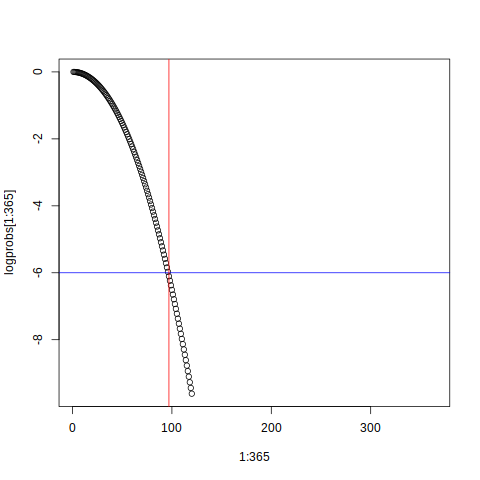
\includegraphics[width=.9\linewidth]{plot.png}
\end{center}
\end{document}